% Author :  Lionel du Peloux
% Contact : lionel.dupeloux@gmail
% Year : 2017

\newrefsegment
\chapter{This is a very very very very very very long title}

\section{This is a very very very very very very long section}
%===================

This chapter is meant to define and introduce what elastic gridshell structures are. It develops a comprehensive but precise view of the numerous knowledge and know-how that gravitate around this concept.

\kant[1-26]


%% two-spreads image
\cleartoleftpage
\begin{tikzpicture}[remember picture,overlay, inner sep=0pt]
	\node[anchor=north west, xshift=-0.5\pgflinewidth, yshift=0.5\pgflinewidth] at (current page.north west){
	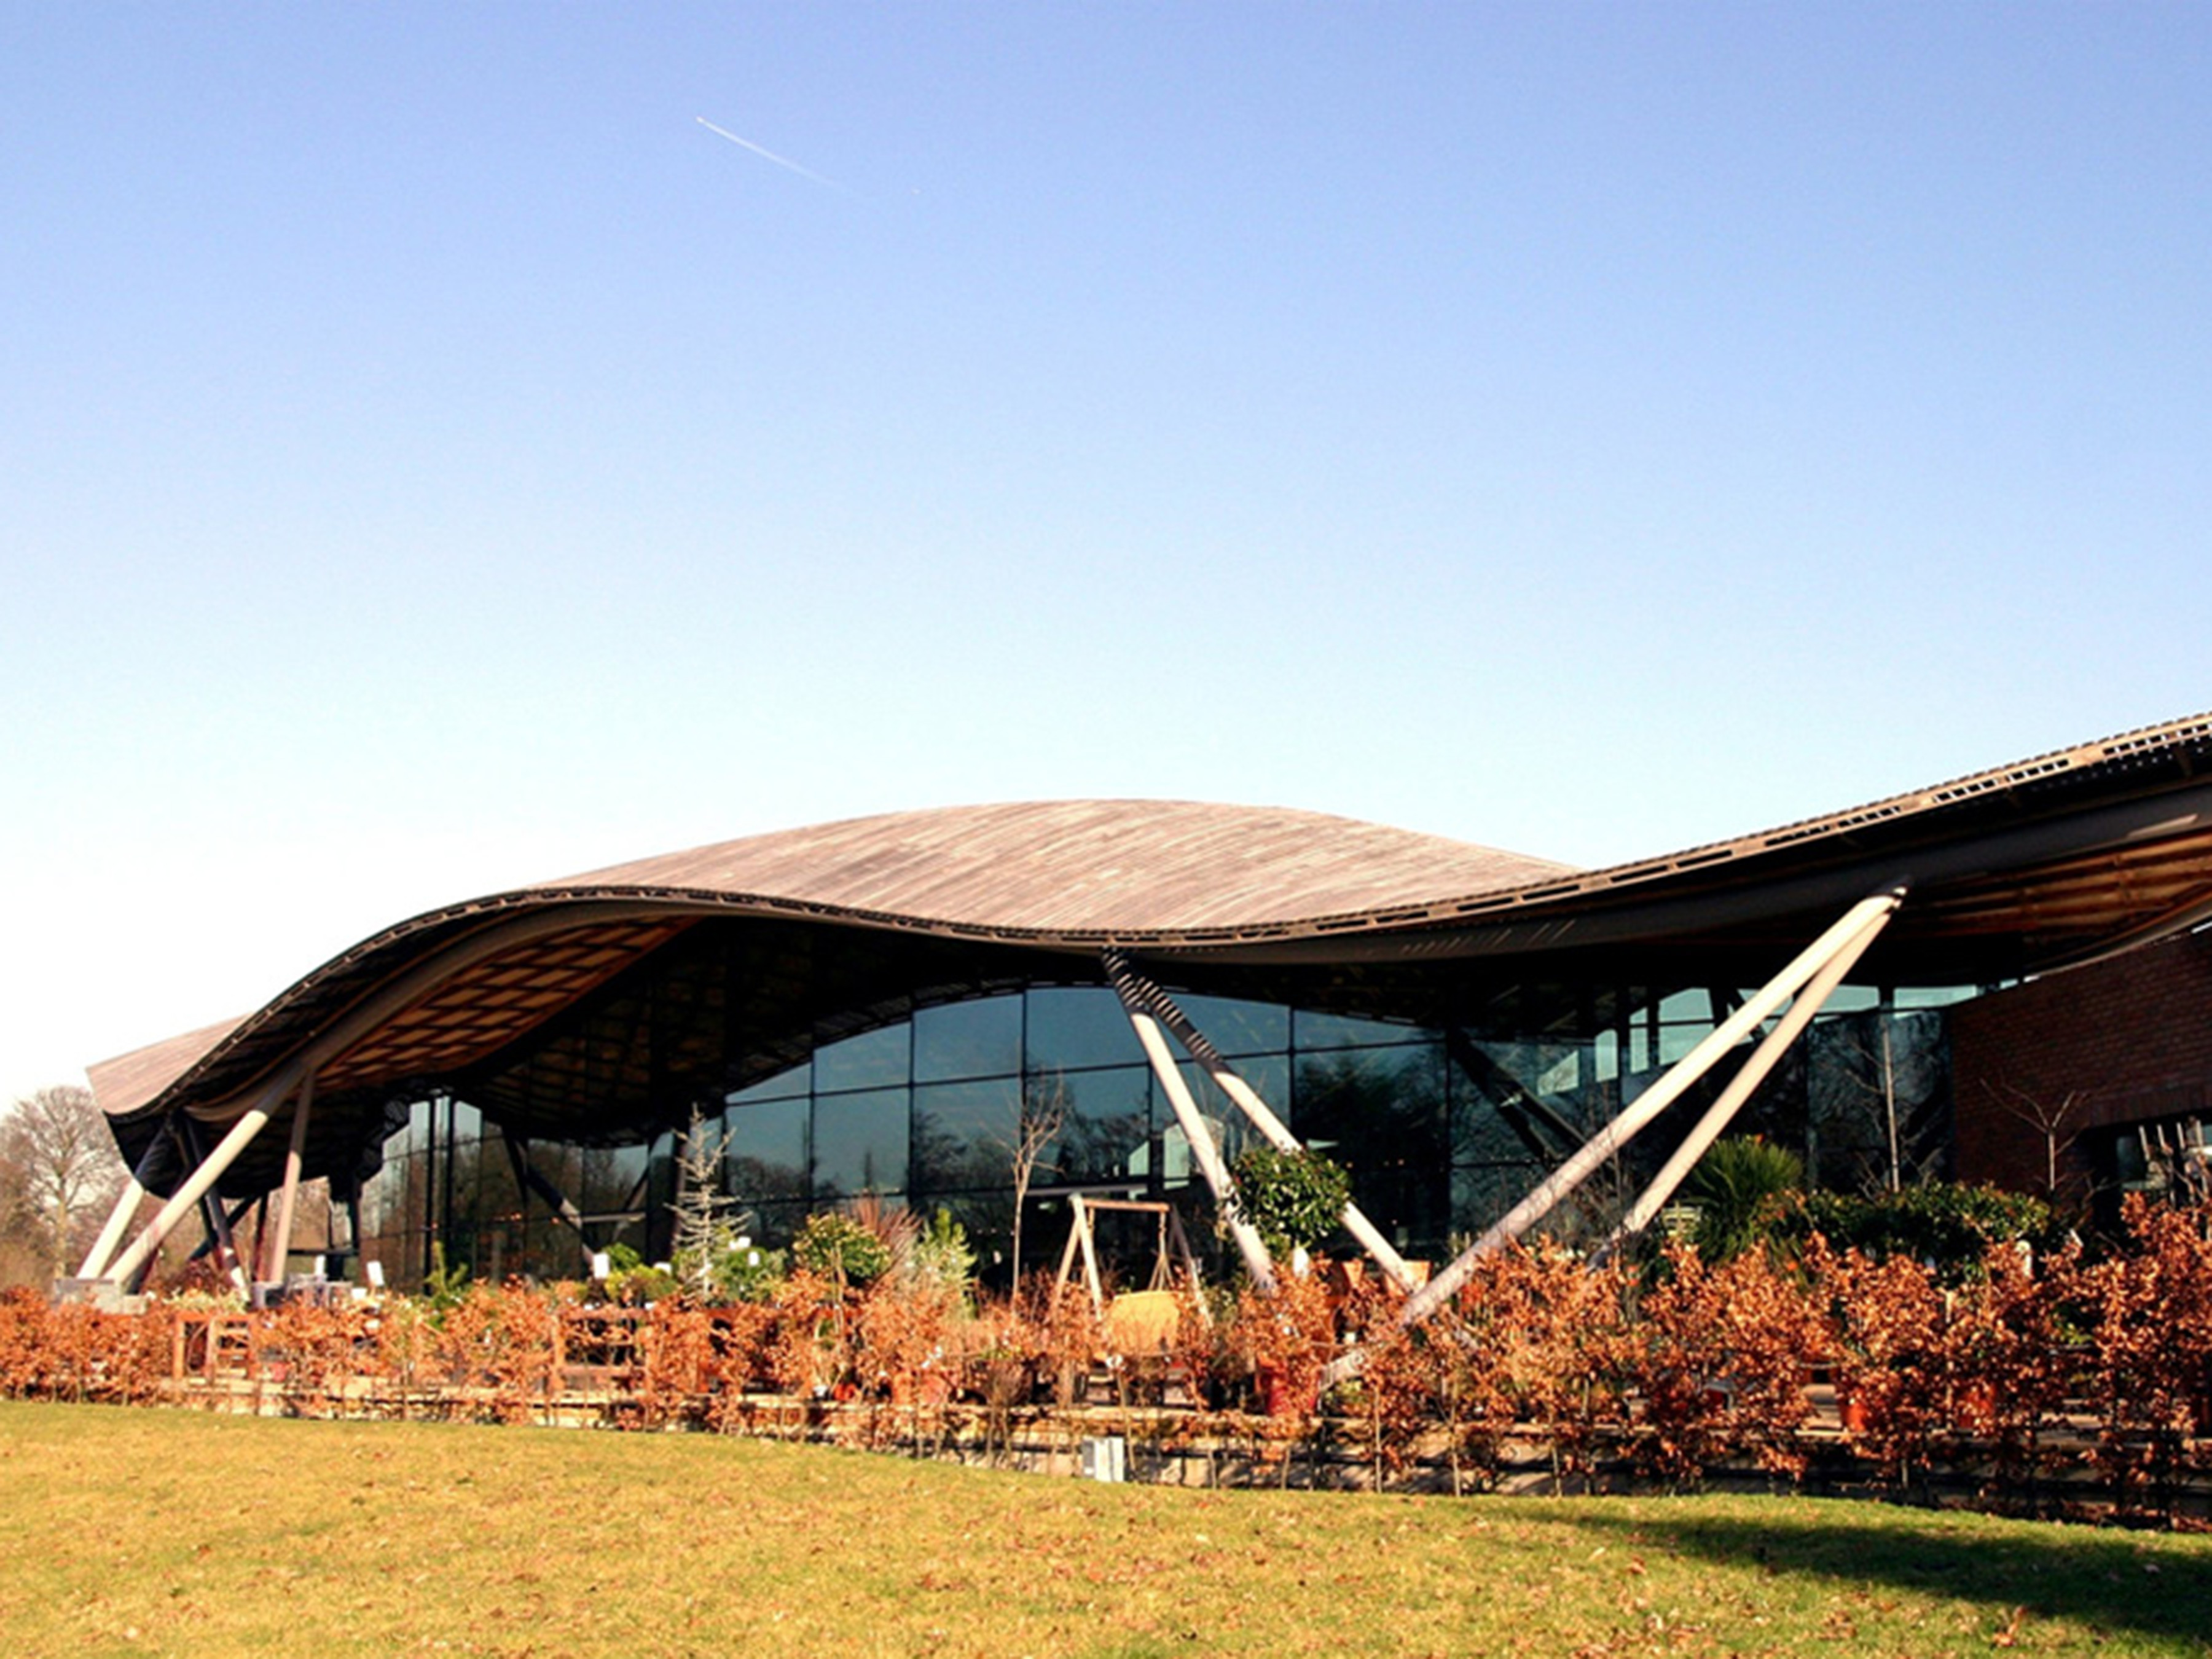
\includegraphics[width=2\paperwidth]{savill_a.jpg}};
\end{tikzpicture}
\clearpage
\begin{tikzpicture}[remember picture,overlay, inner sep=0pt]
	\node[anchor=north west, xshift=-0.5\pgflinewidth-\paperwidth, yshift=0.5\pgflinewidth] at (current page.north west){
	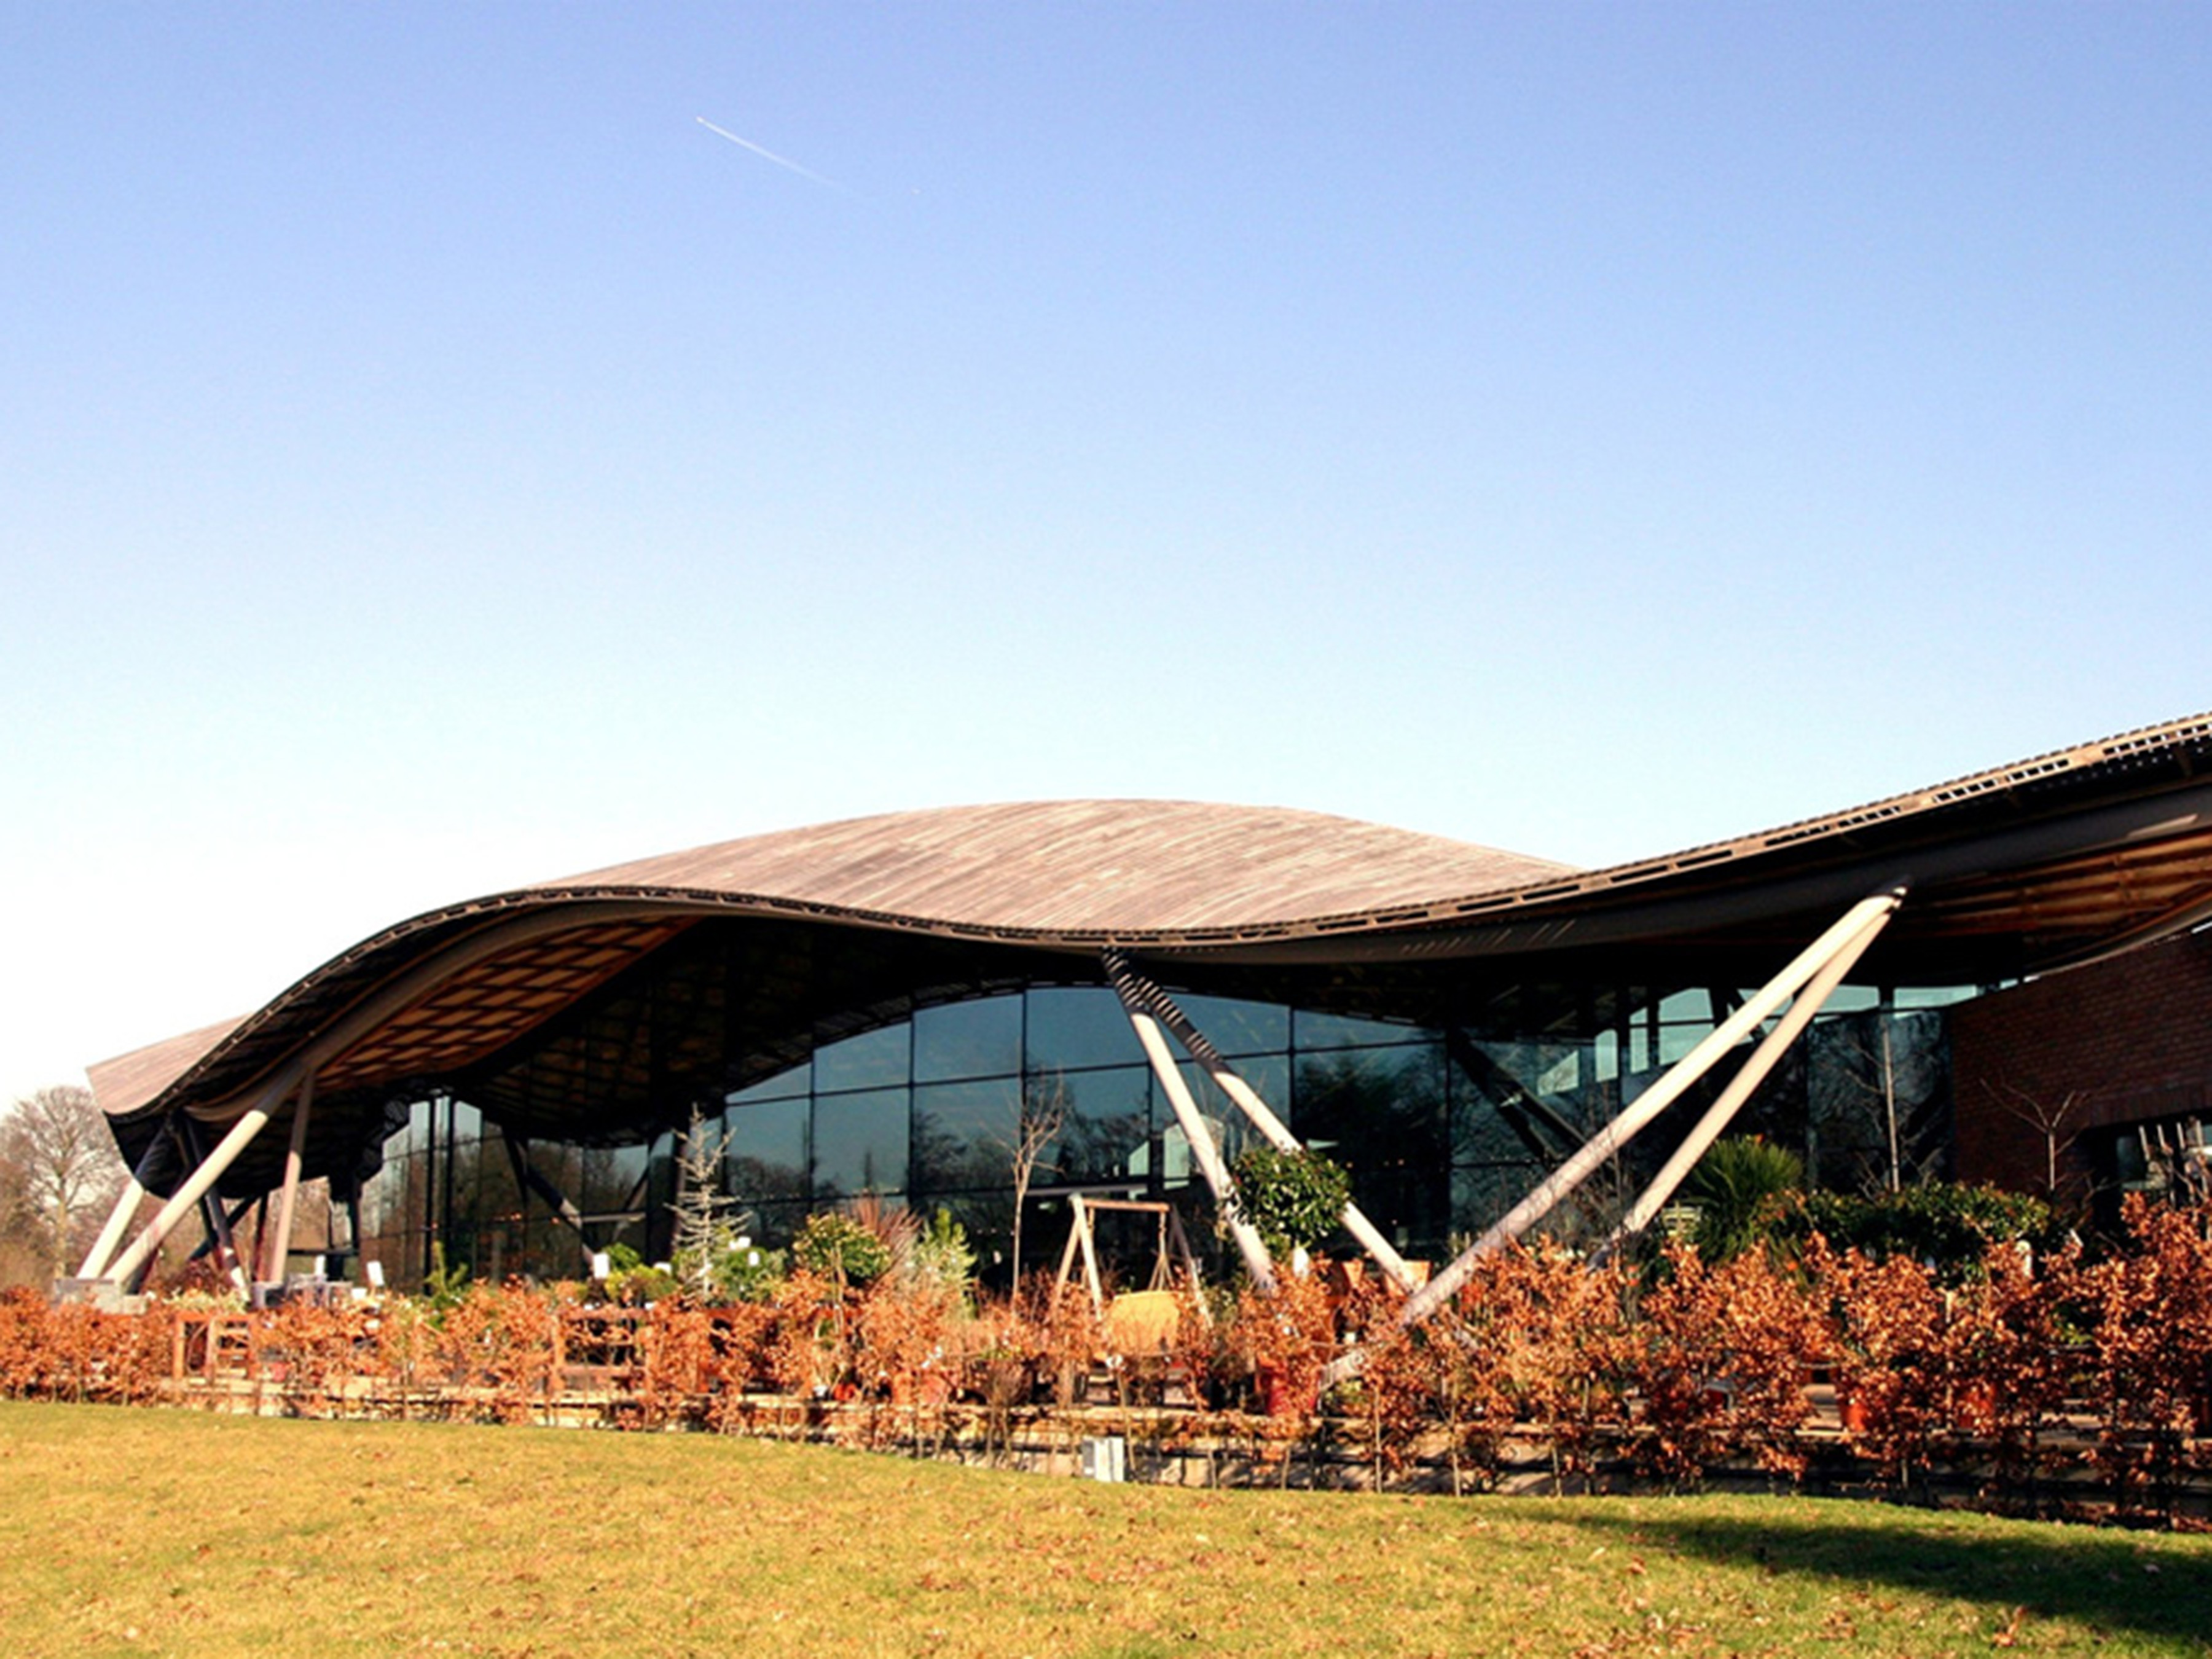
\includegraphics[width=2\paperwidth]{savill_a.jpg}};
\end{tikzpicture}


%%%%%%%%%%%%%
\clearpage
\kant[1-2]

\cleartoleftpage
\begin{textblock*}{10cm}[0,0](0cm,0cm)\noindent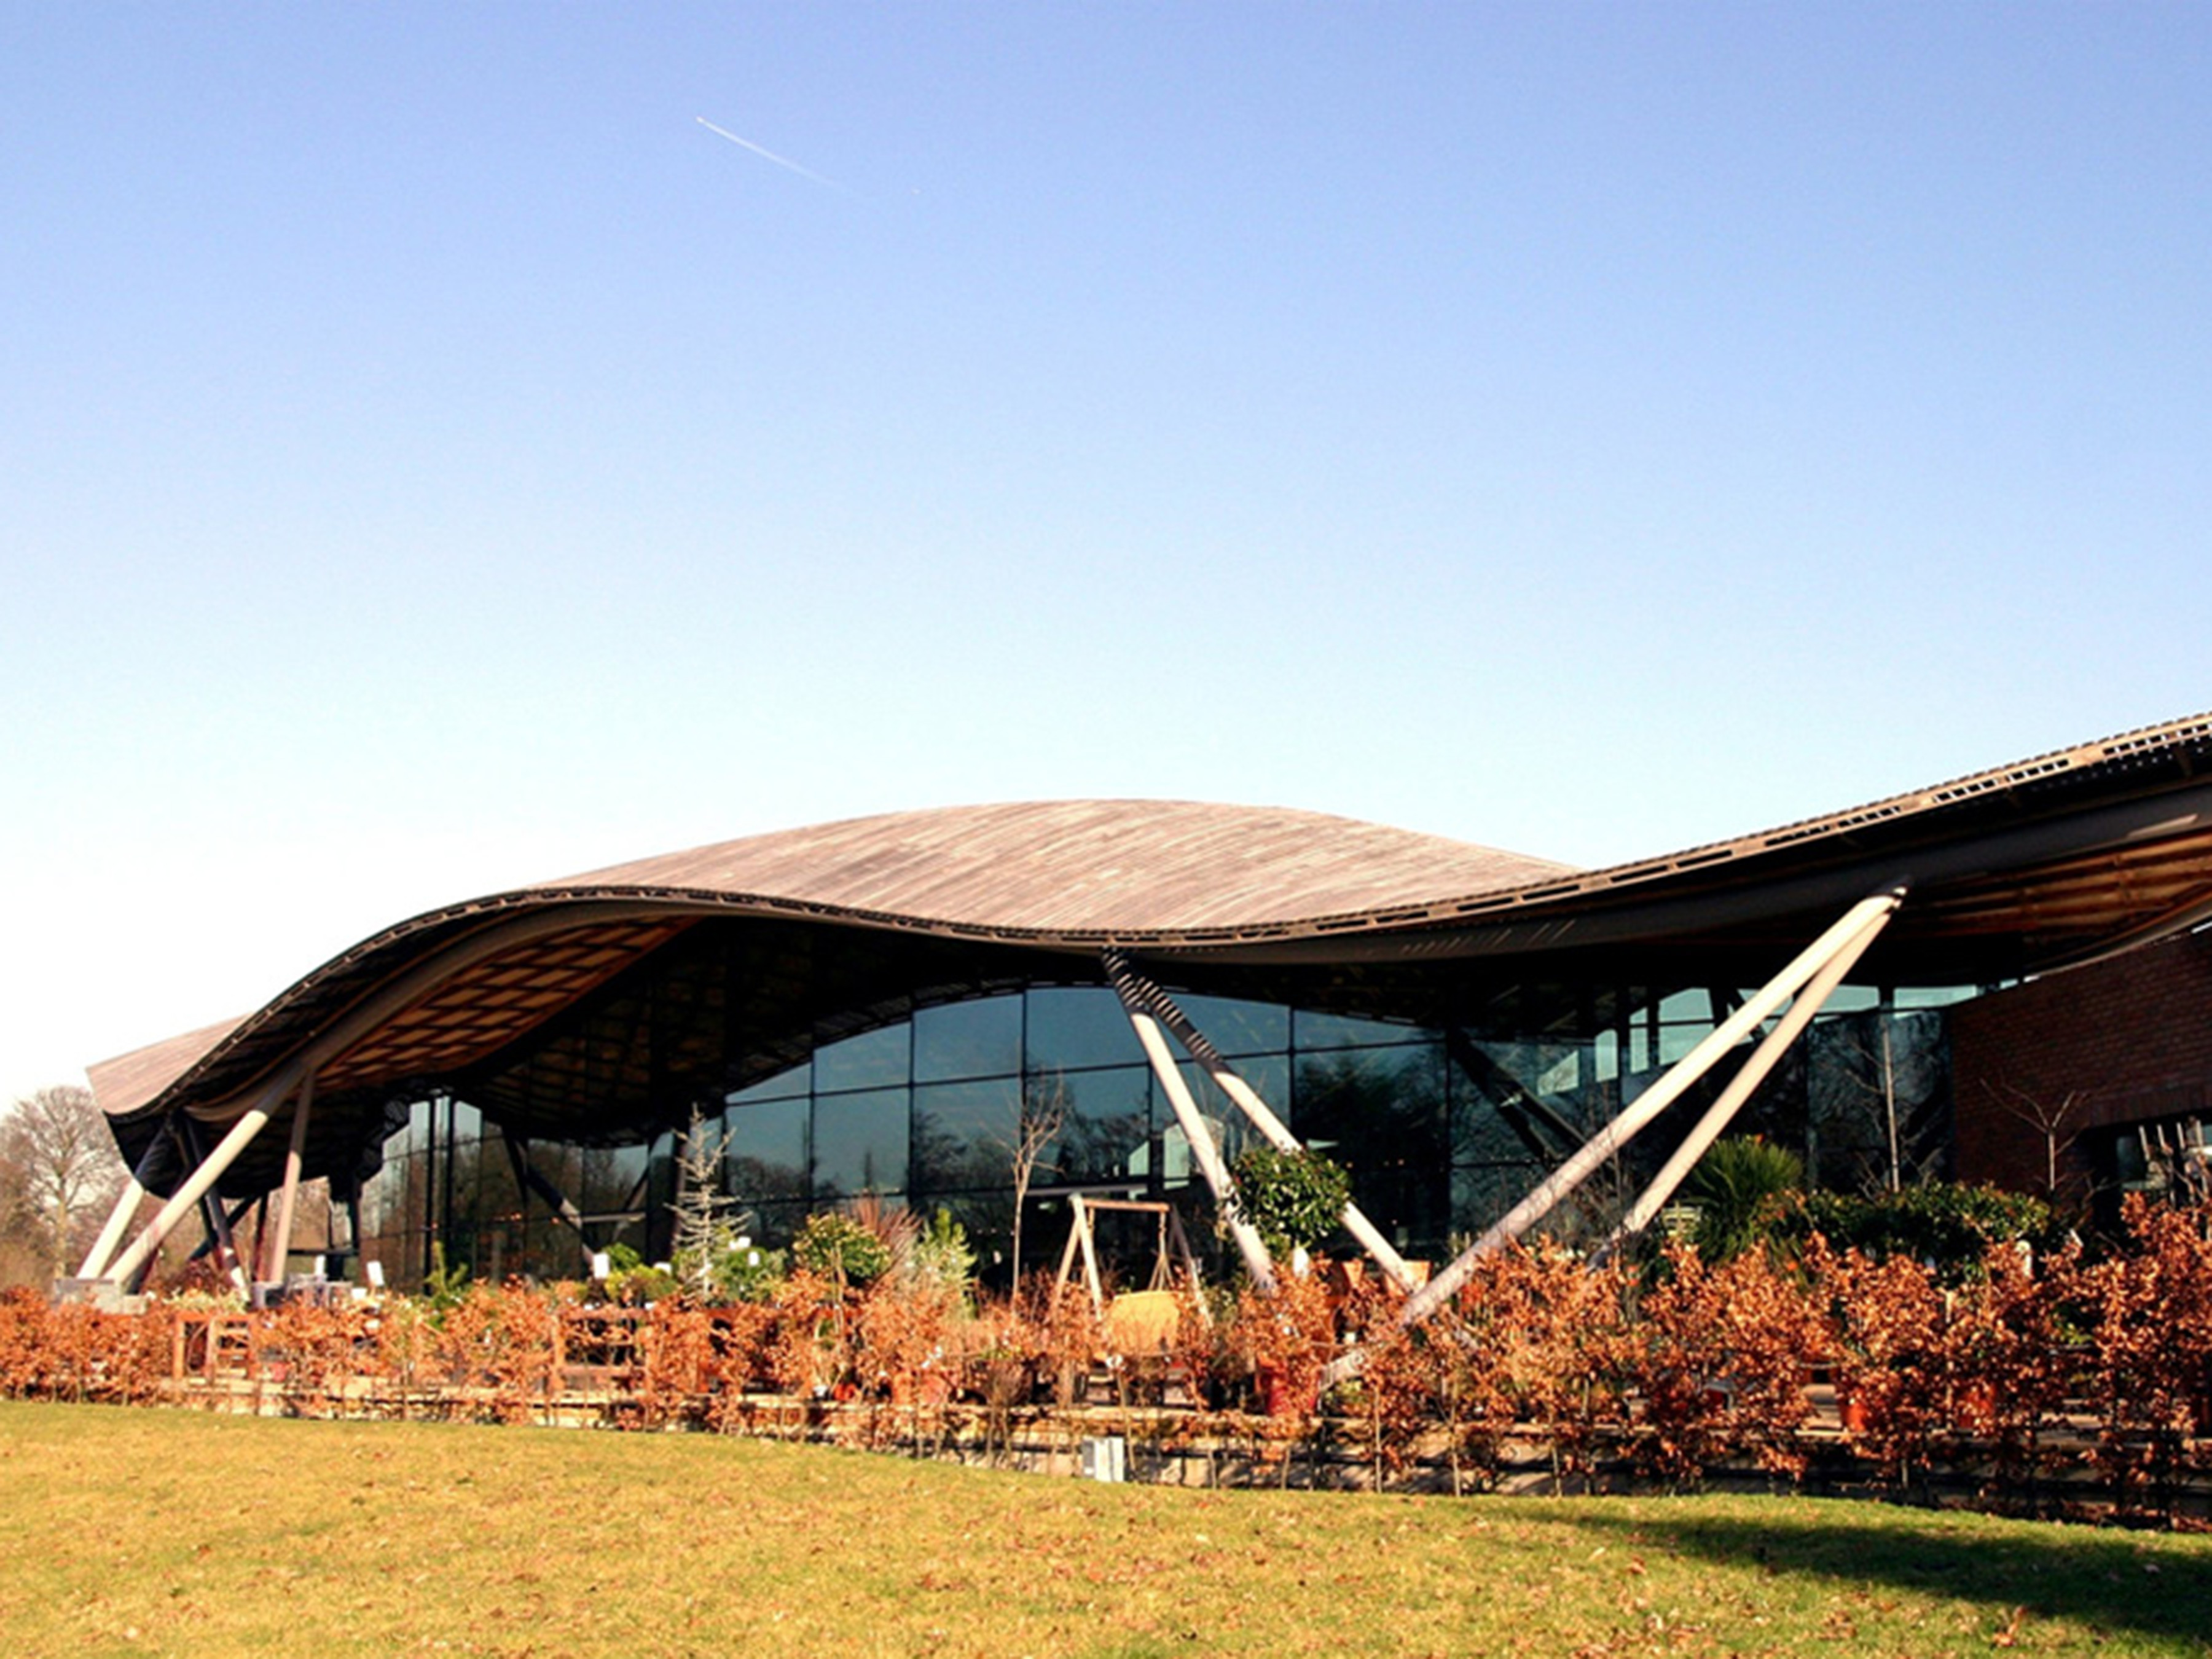
\includegraphics[width=10cm]{savill_a.jpg}\end{textblock*}


% \clearpage
% skdmlskdmslkd
% \begin{tikzpicture}[remember picture,overlay,inner sep=0pt]
% 	\node[anchor=north east,inner sep=0pt] at (current page.north east)
% 	{
% 	\begin{minipage}{\paperwidth}
% 		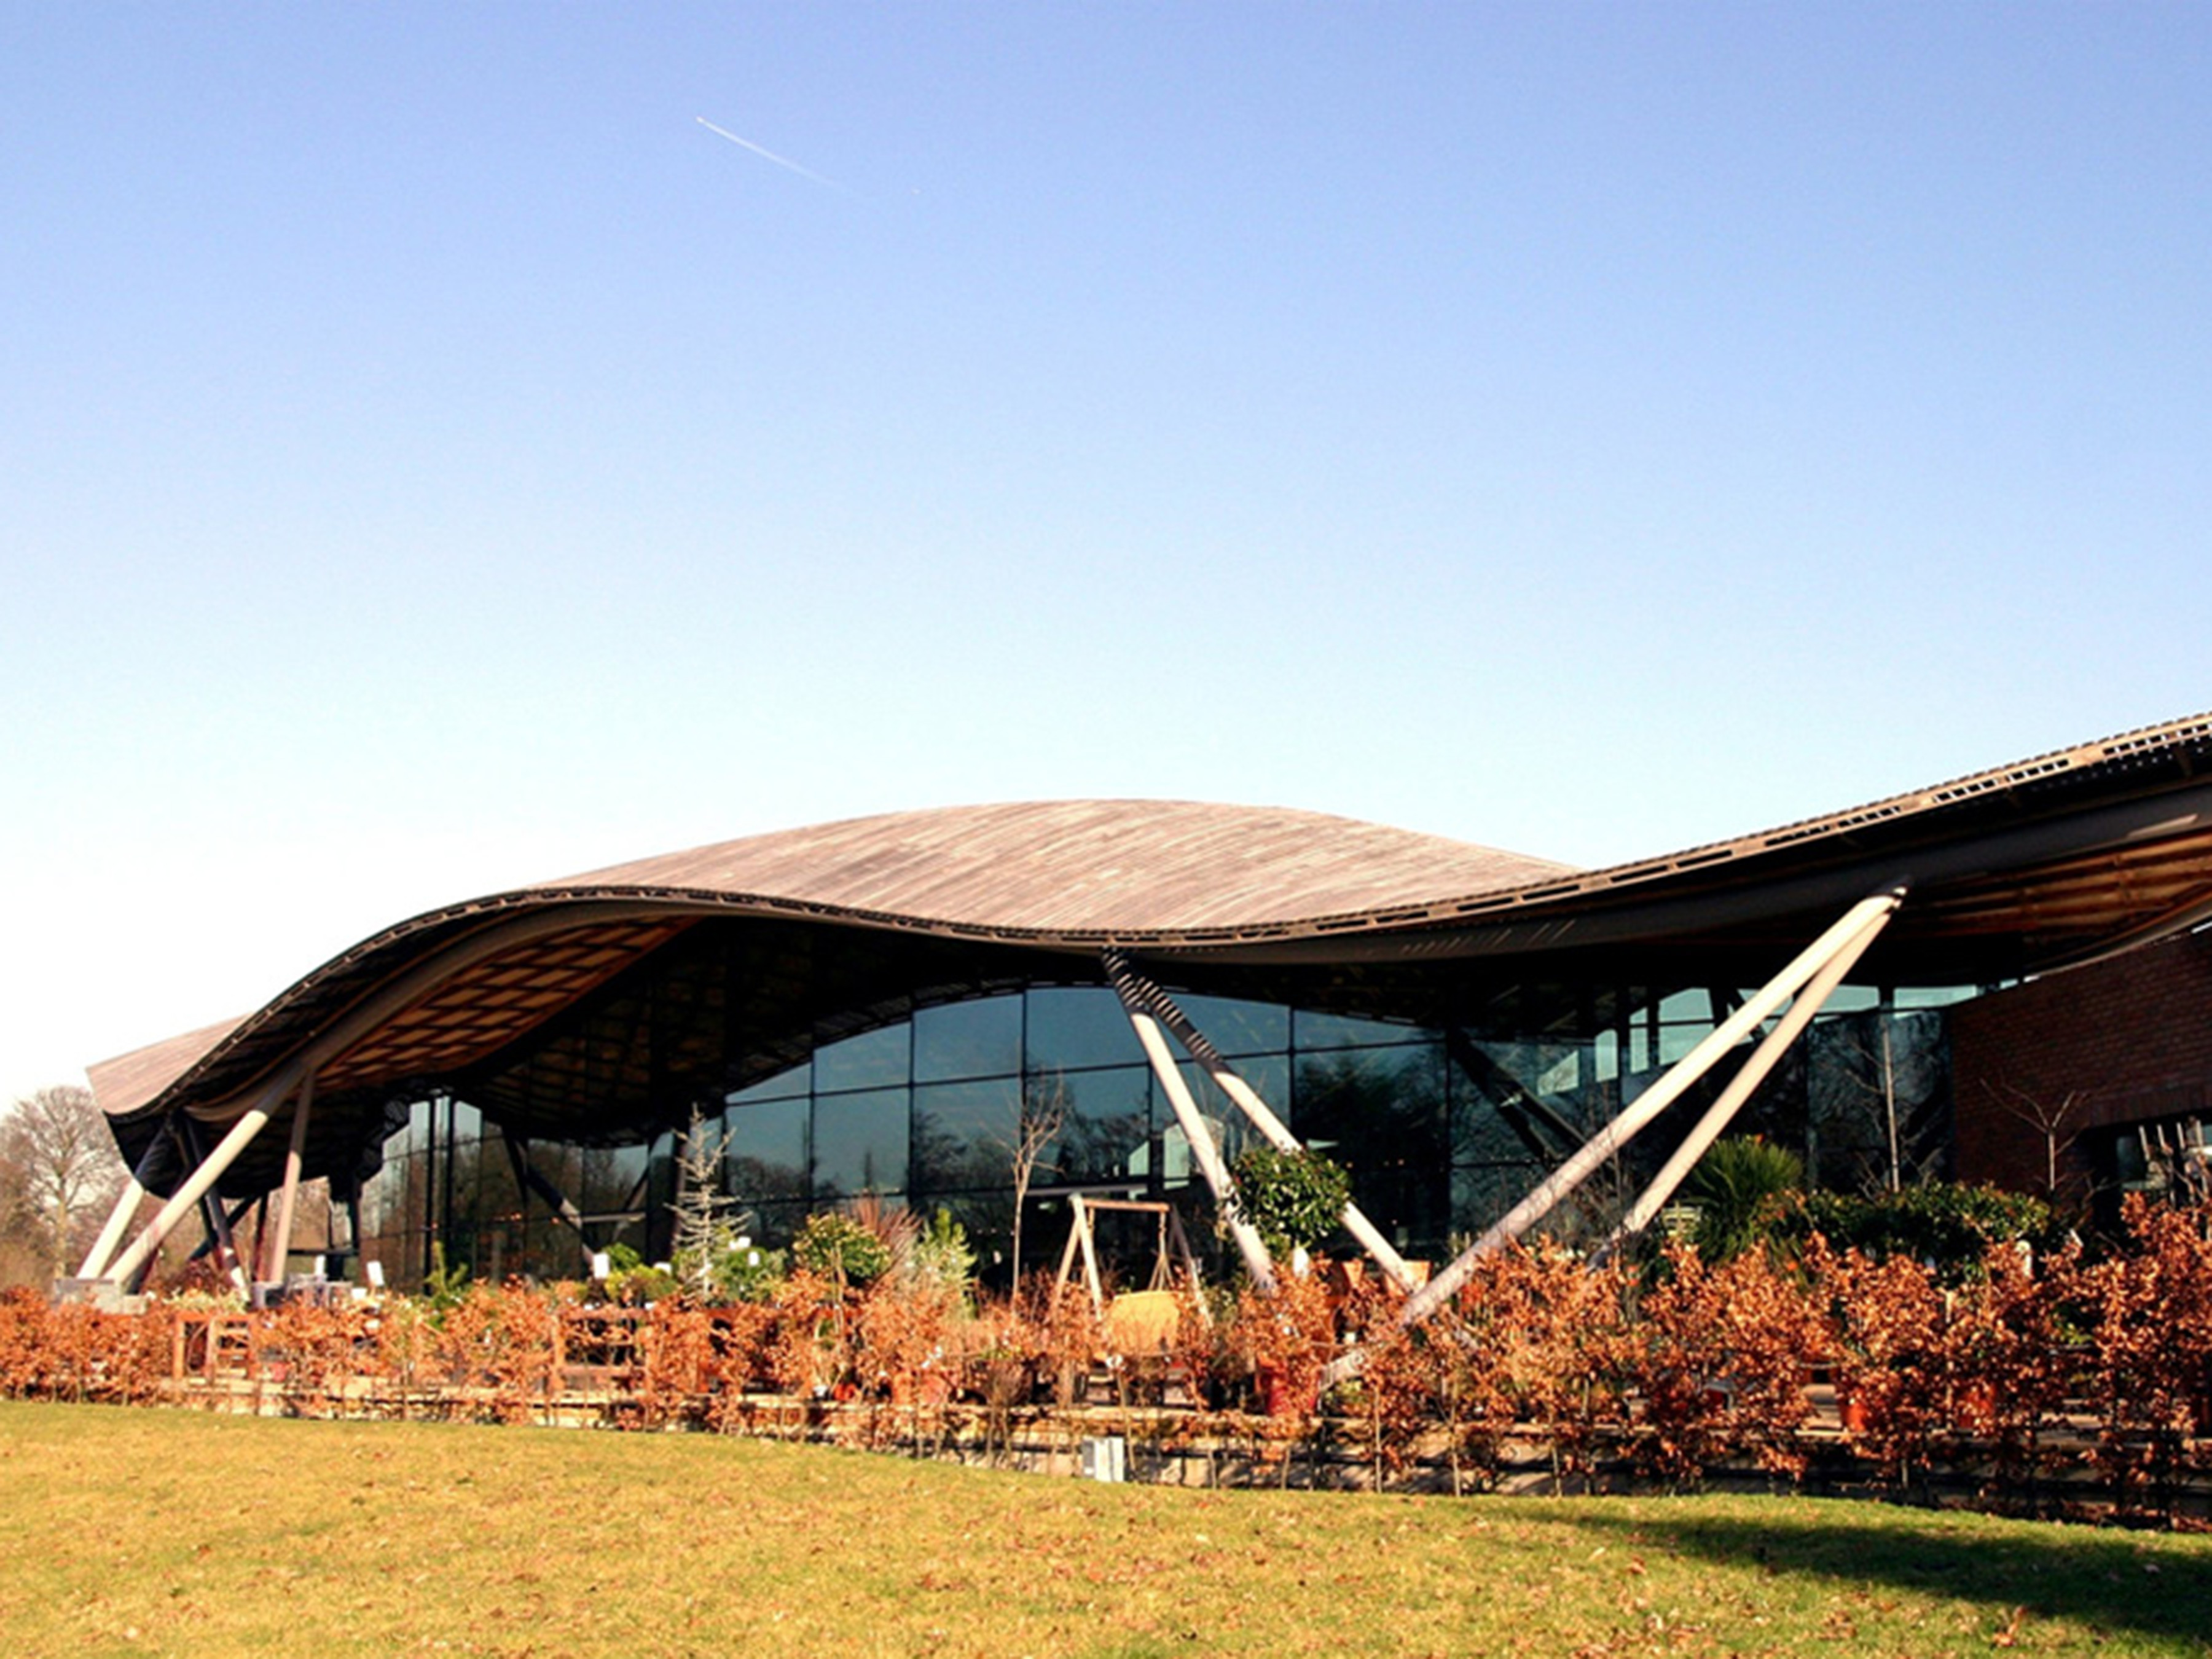
\includegraphics[width=\paperwidth]{savill_a.jpg}
% 		\captionof{figure}{sdsdksdmskdms}
% 	\end{minipage}
% 	};
% \end{tikzpicture}

% \clearpage
% \begin{tikzpicture}[remember picture,overlay]
% 	\node[anchor=north west,inner sep=0pt] at (current page.north west)
% 	{
% 	\begin{minipage}{\textwidth}
% 		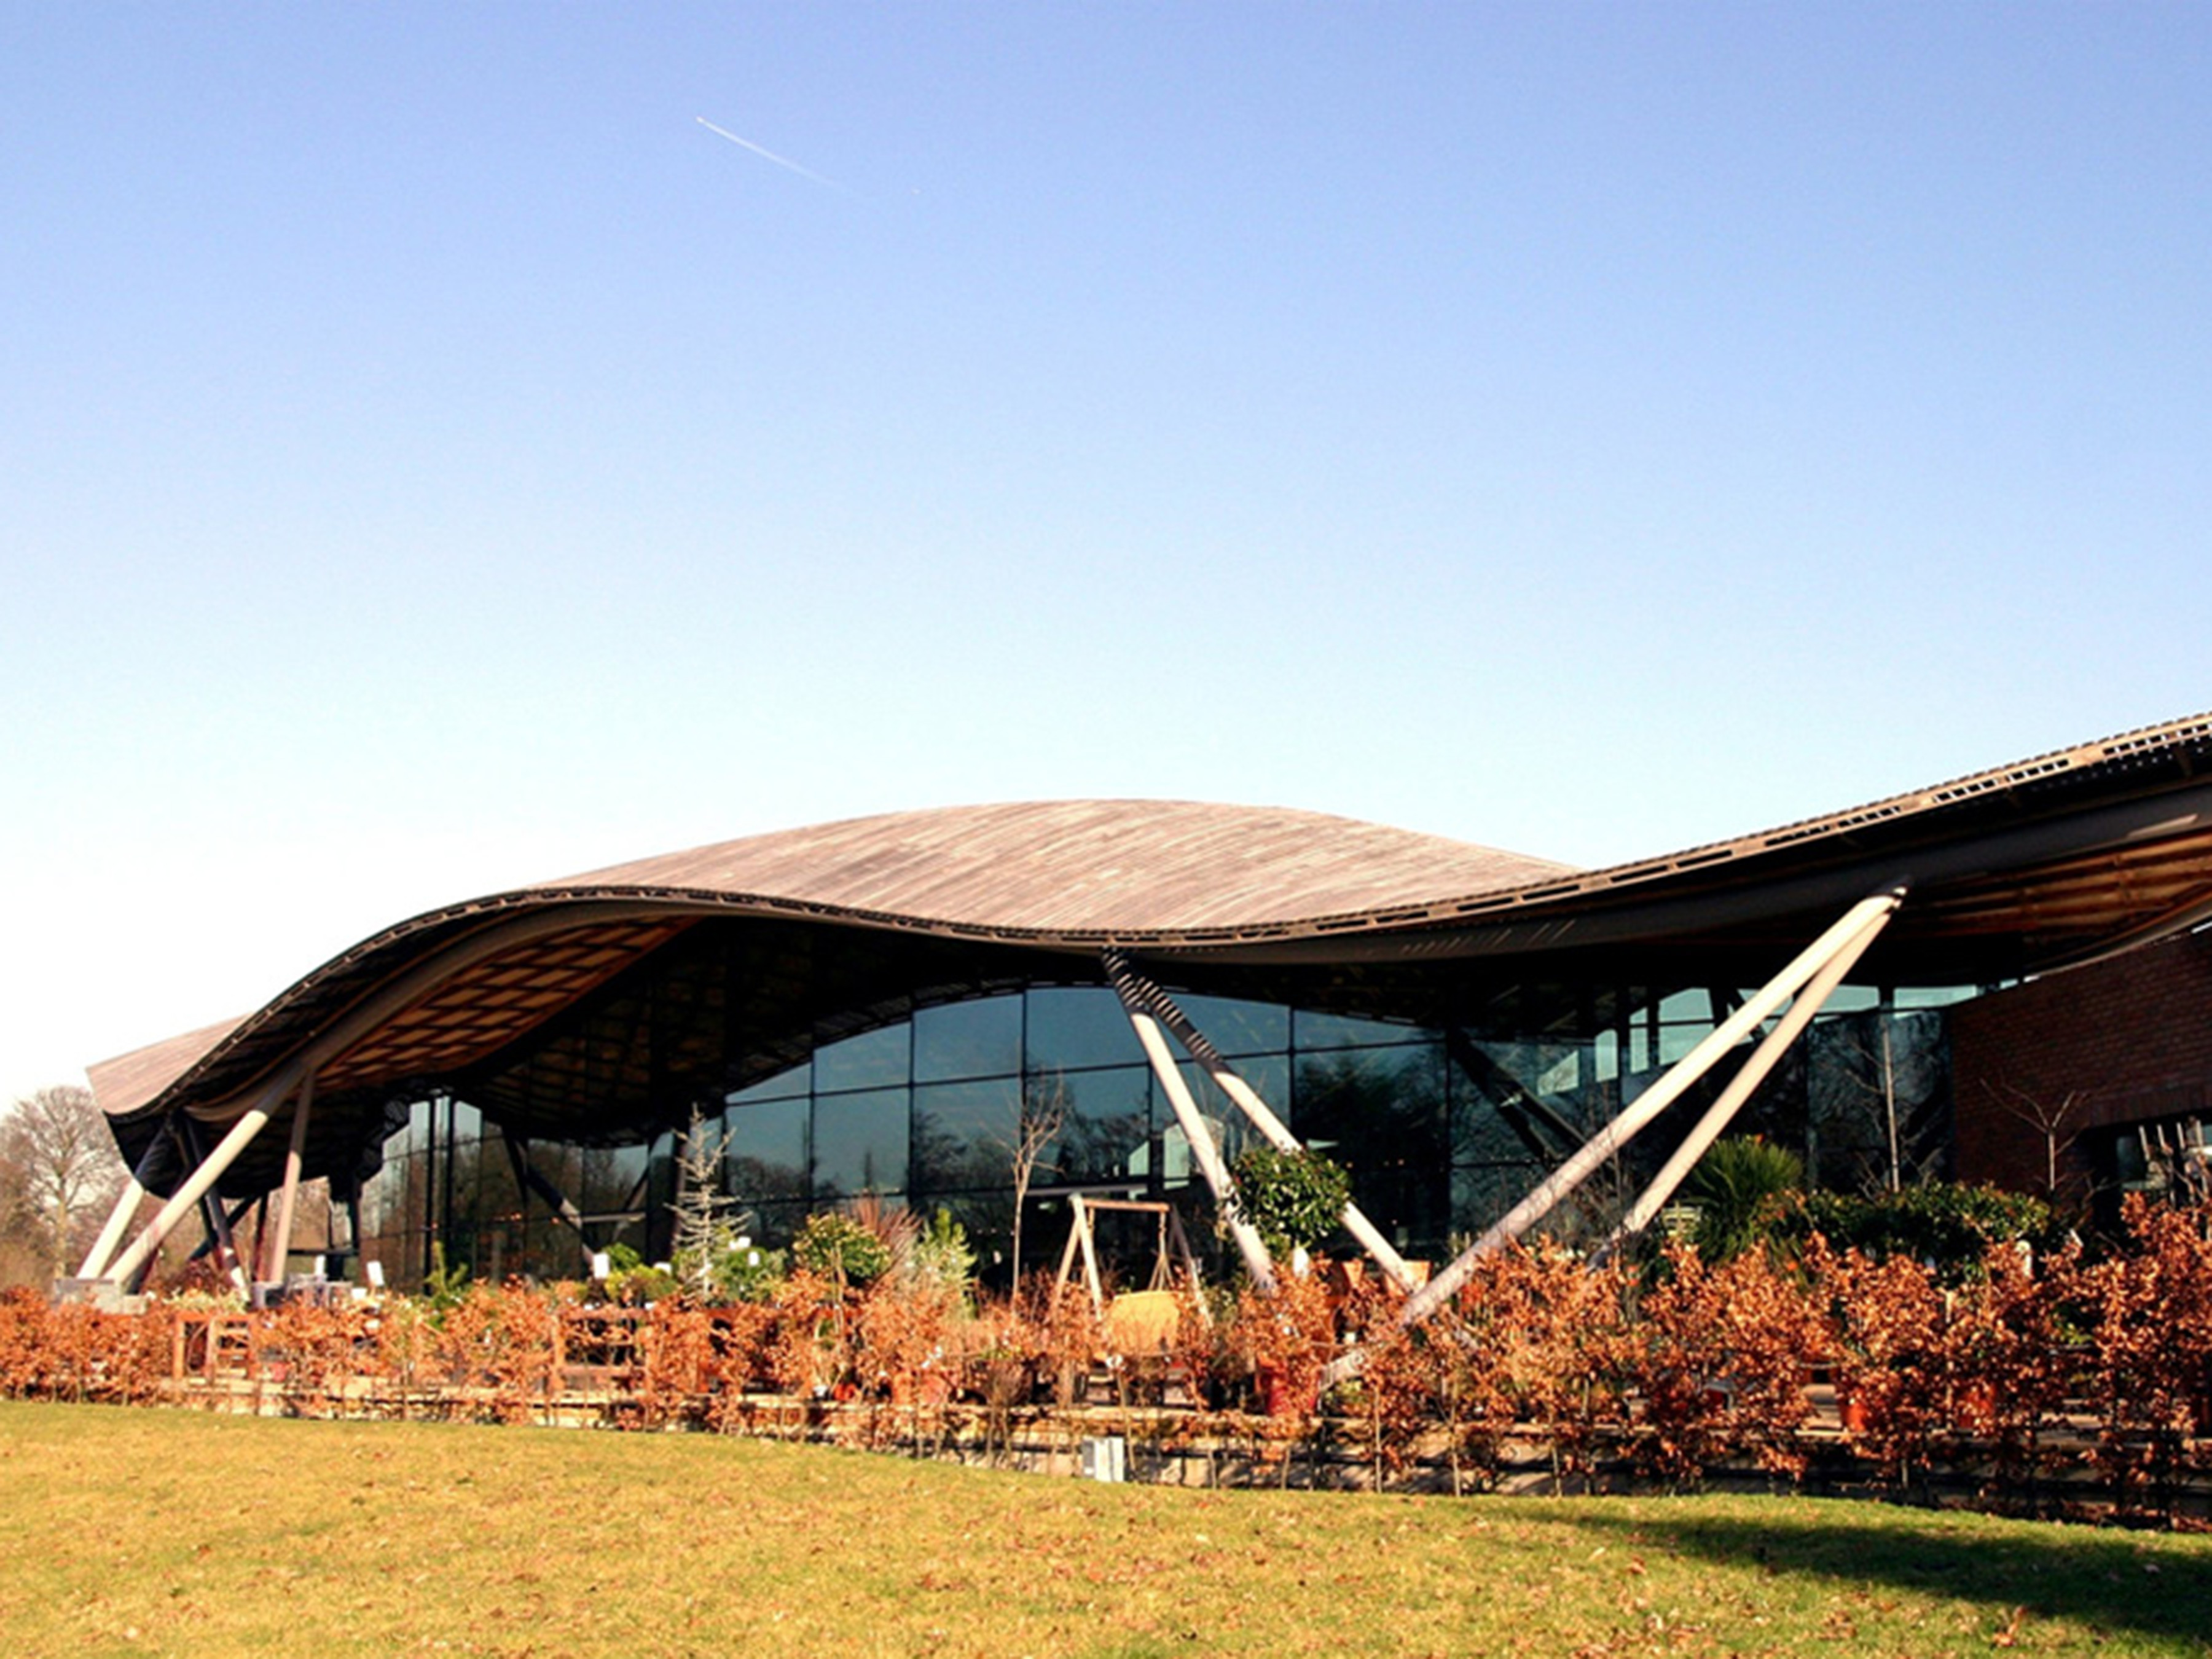
\includegraphics[width=\textwidth]{savill_a.jpg}
% 		\captionof{subfigure}{}{\label{fig:savill_d}}
% 	\end{minipage}
% 	};
% \end{tikzpicture}

% REF : \cref{fig:savill_d}


% \setlength{\unitlength}{1cm}
% % \begin{picture}(50,50)
% % 	\put(0,0){\hbox{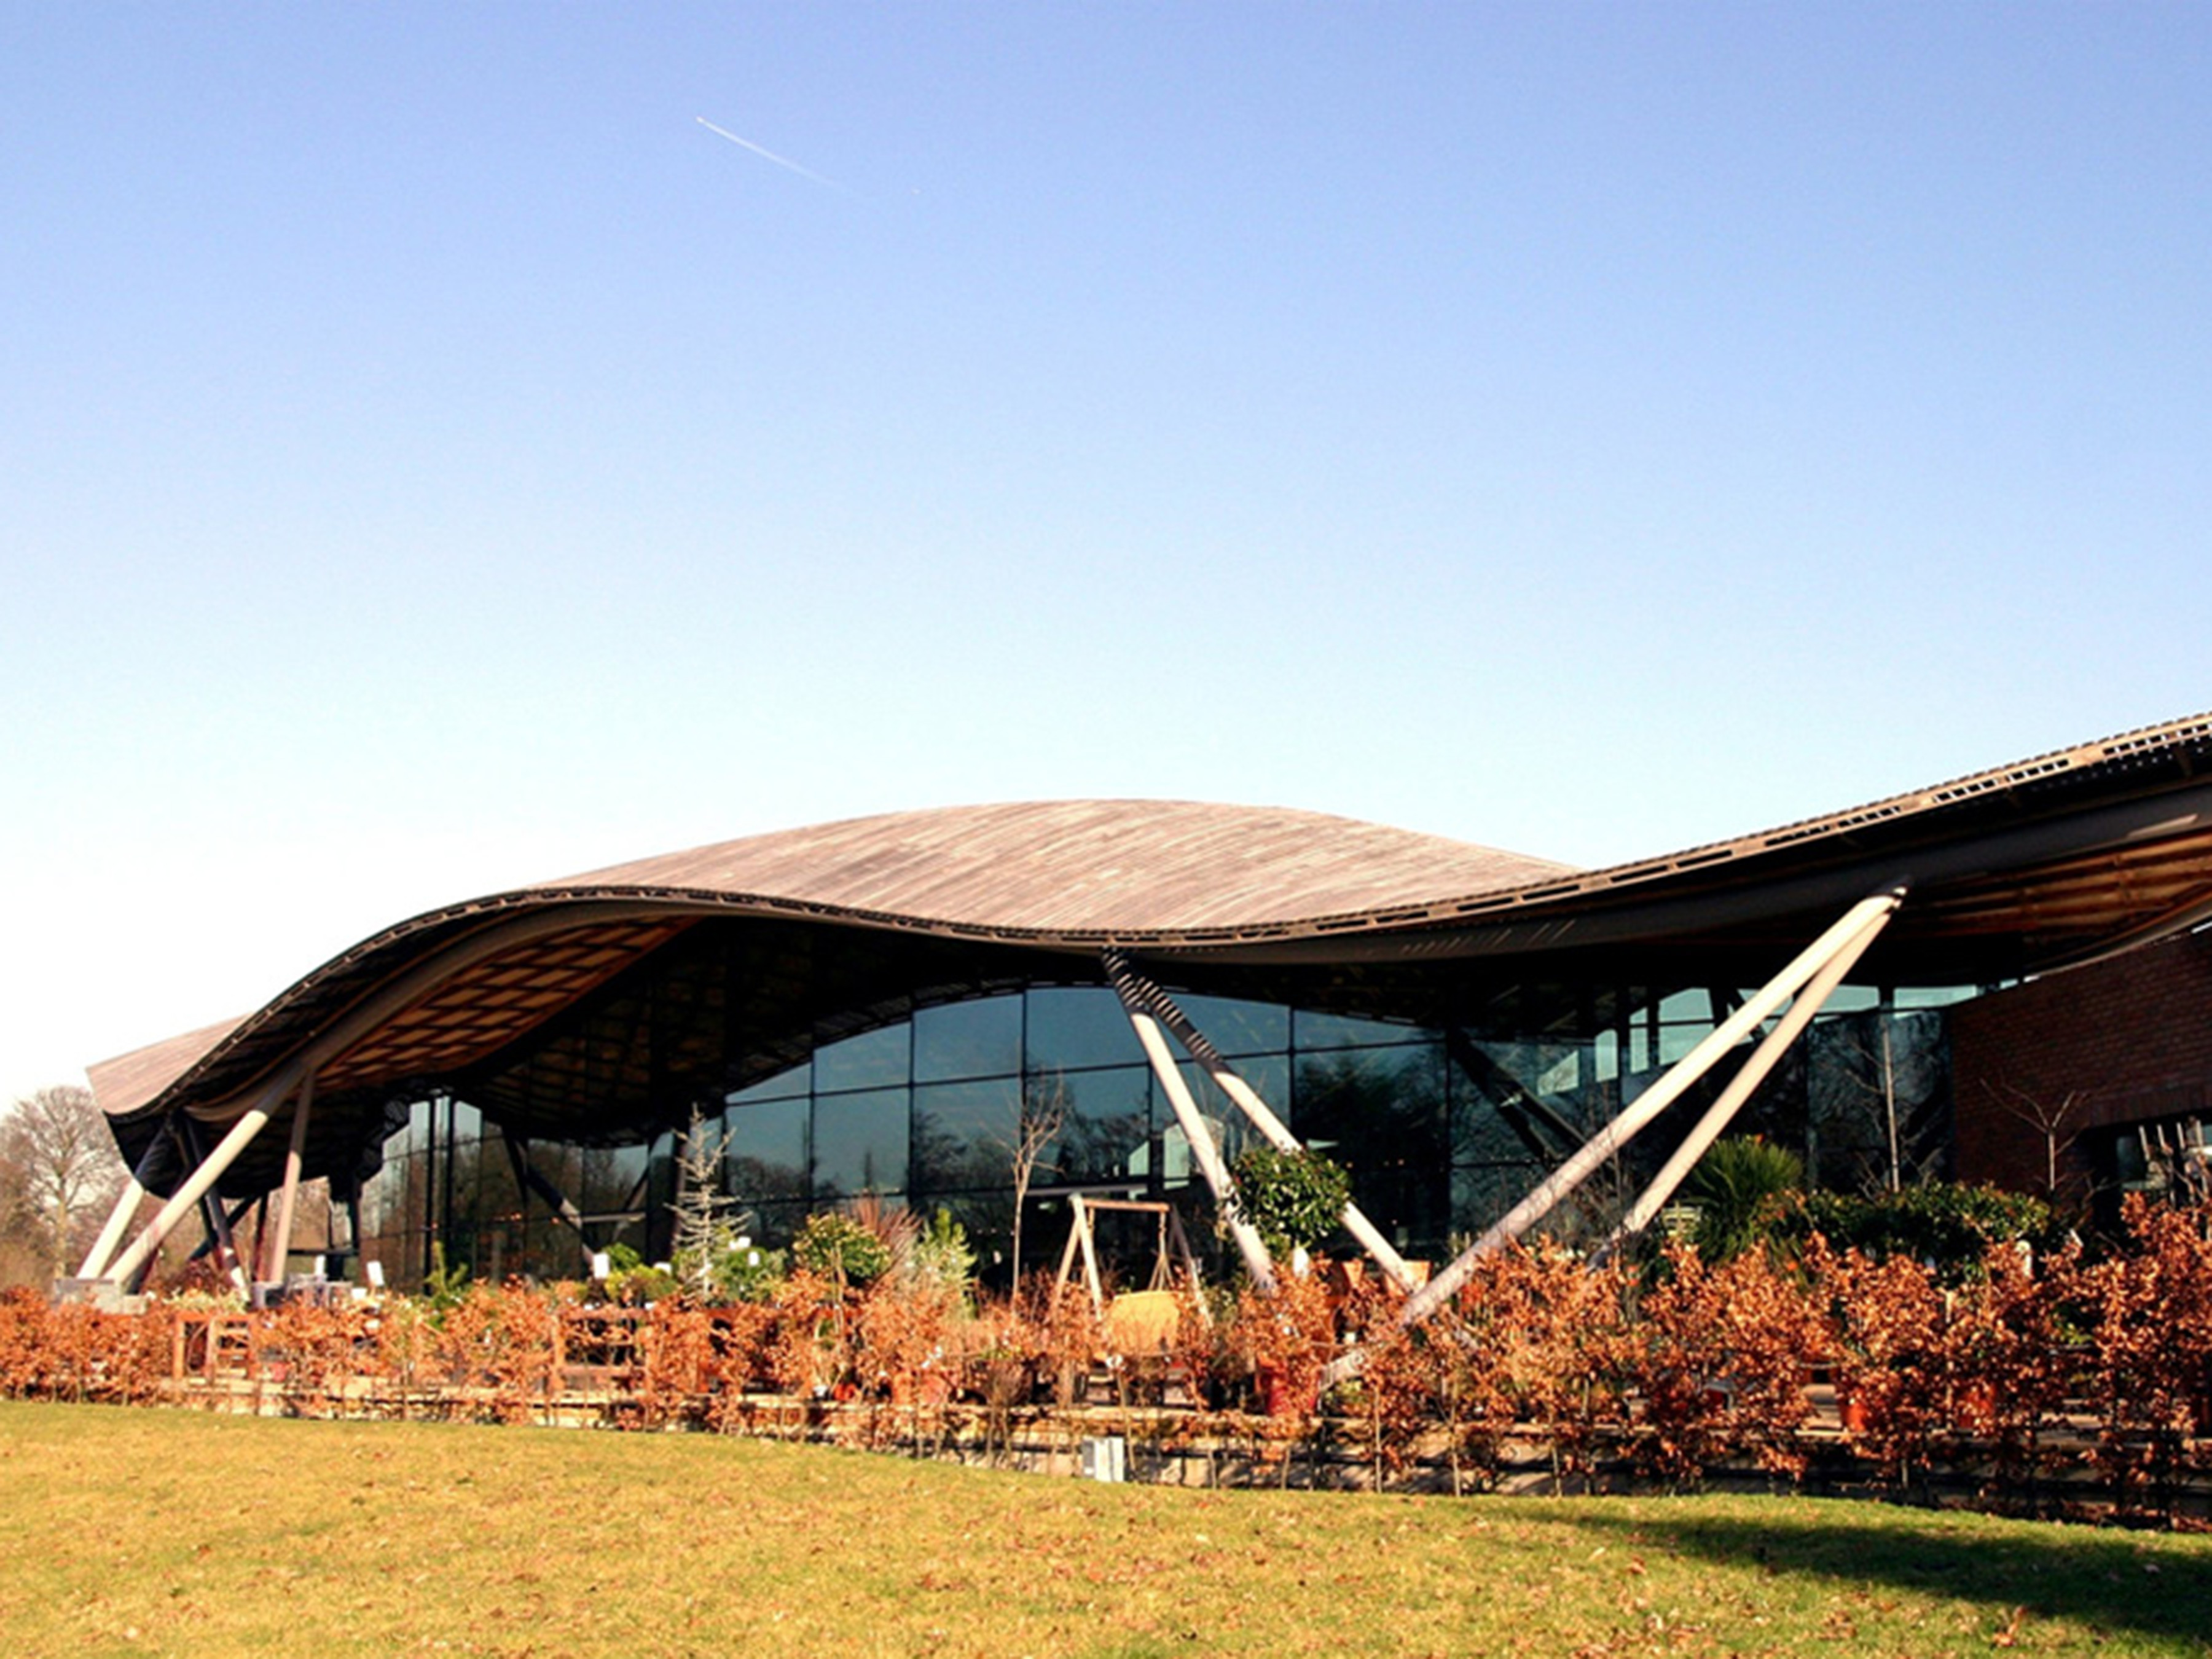
\includegraphics[width=\paperwidth]{savill_a.jpg}}}
% % \end{picture}

% \begin{picture}(0,-10)
% \put(0,0){%
% \begin{minipage}{0.48\linewidth}
% 	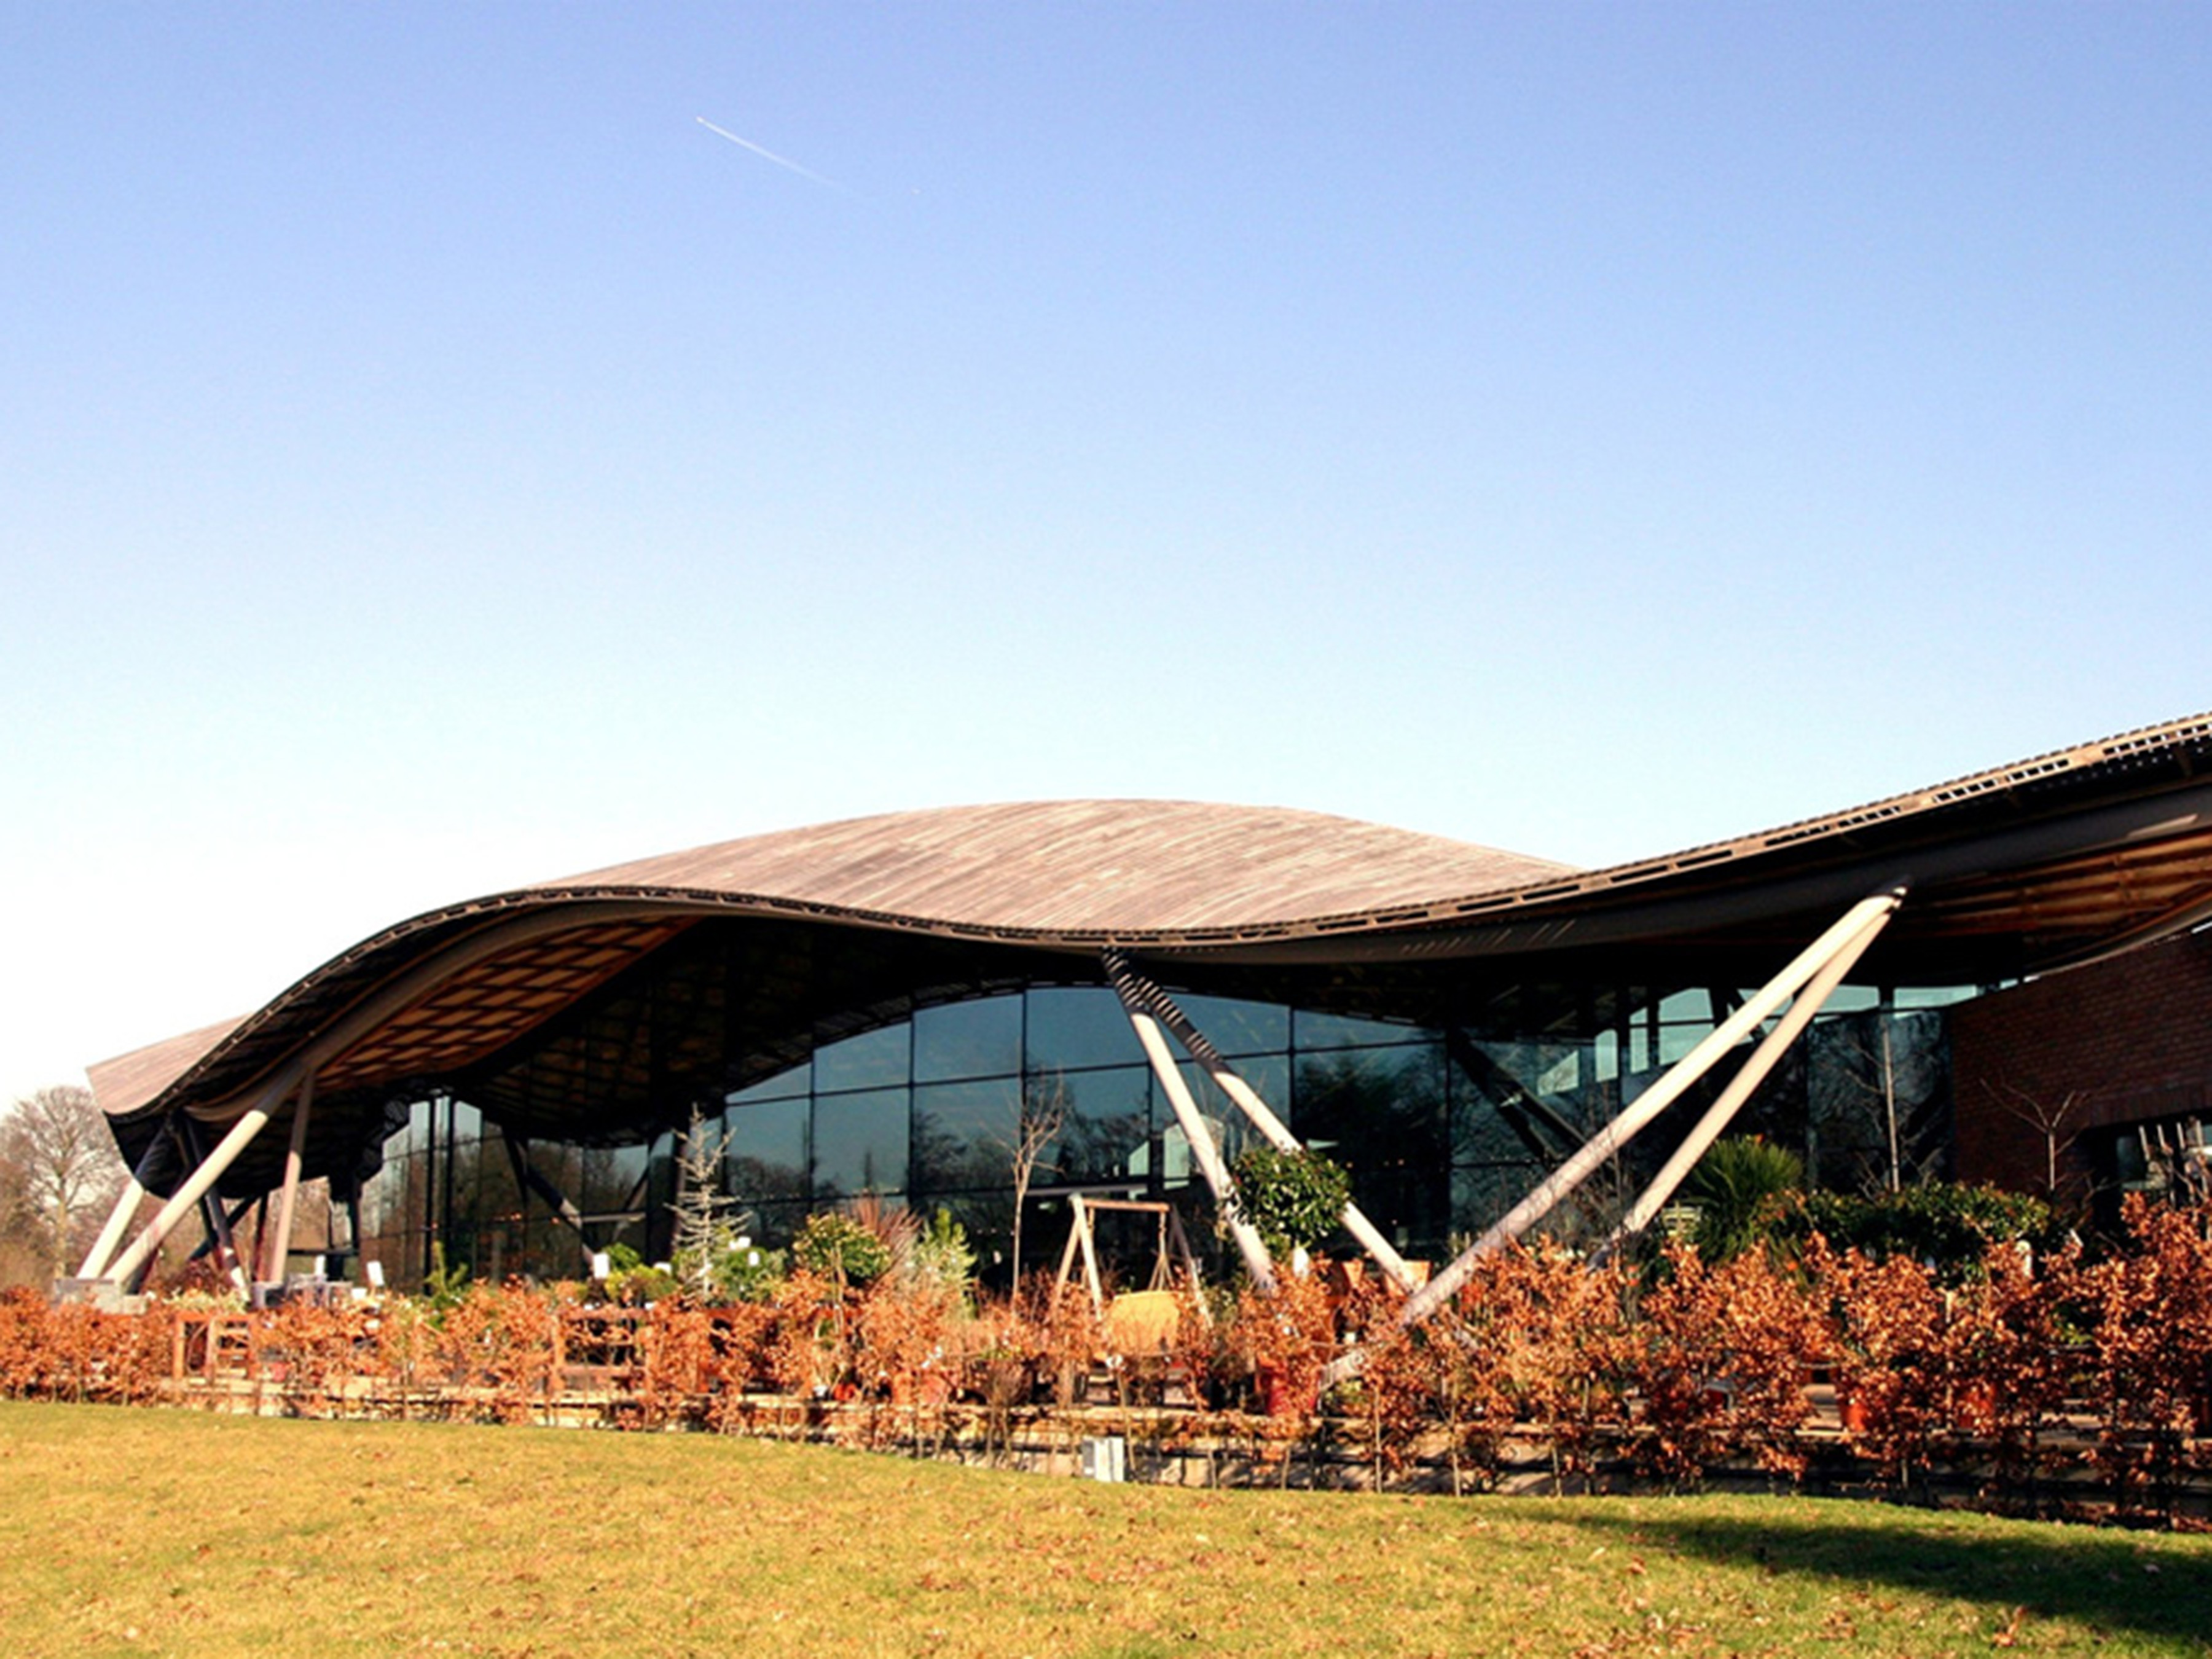
\includegraphics[width=\linewidth]{savill_a.jpg}
% 	\captionof{figure}{Some here}
% \end{minipage}%
% }
% \end{picture}

%  \begin{textblock}{2.5}(\GetX{2cm},\GetY{0cm})
% 	\raggedright
% 	Work is of two kinds: first, altering
% 	the position of matter at or near the
% 	earth’s surface relatively to other such
% 	matter; second, telling other people
% 	to do so.
% \end{textblock}

% \begin{textblock*}{10cm}[0,0](0cm,0cm)
% 	\raggedright
% 	Work is of two kinds: first, altering
% 	the position of matter at or near the
% 	earth’s surface relatively to other such
% 	matter; second, telling other people
% 	to do so.
% \end{textblock*}
